
\newcommand{\imagewidth}{2.3cm}
\newcommand{\imageheight}{3.5263671874999996cm}
\newcommand{\smallimagewidth}{0.8cm}
\newcommand{\smallimageheight}{1.2265625cm}
\newcommand{\borderthickness}{0.41pt}
\def\myshift#1{\raisebox{0.5ex}}
\renewcommand{\teasernobox}{
  \begin{subfigure}[b]{\linewidth}
    \centering
    \resizebox{\linewidth}{!}{
      \begin{tikzpicture}[
          >=stealth',
          overlay/.style={
              anchor=south west,
              draw=black,
              rectangle,
              line width=0.8pt,
              outer sep=0,
              inner sep=0,
            },
        ]
        \small
        \matrix[matrix of nodes, column sep=1pt, row sep=1pt, ampersand replacement=\&, inner sep=0, outer sep=0] (training) {
          \includegraphics[height=\imageheight]{assets/\blendfieldsdirname/teaser2/voltemorph/0000_mix.png} \&
          \includegraphics[height=\imageheight]{assets/\blendfieldsdirname/teaser2/voltemorph/0001_mix.png} \&
          \includegraphics[height=\imageheight]{assets/\blendfieldsdirname/teaser2/voltemorph/0003_mix.png} \&
          \includegraphics[height=\imageheight]{assets/\blendfieldsdirname/teaser2/voltemorph/0004_mix.png} \&
          \includegraphics[height=\imageheight]{assets/\blendfieldsdirname/teaser2/voltemorph/0007_mix.png} \\
          \includegraphics[height=\imageheight]{assets/\blendfieldsdirname/teaser2/ours/0000_mix.png} \&
          \includegraphics[height=\imageheight]{assets/\blendfieldsdirname/teaser2/ours/0001_mix.png} \&
          \includegraphics[height=\imageheight]{assets/\blendfieldsdirname/teaser2/ours/0003_mix.png} \&
          \includegraphics[height=\imageheight]{assets/\blendfieldsdirname/teaser2/ours/0004_mix.png} \&
          \includegraphics[height=\imageheight]{assets/\blendfieldsdirname/teaser2/ours/0007_mix.png}       \\
        };
        \node[above right=\borderthickness and \borderthickness of training-2-1.south west, overlay]{
          
\includegraphics[height=\smallimageheight]{assets/\blendfieldsdirname/teaser2/colorsv2/0000.png}
        };
        \node[above right=\borderthickness and \borderthickness of training-2-2.south west, overlay]{
          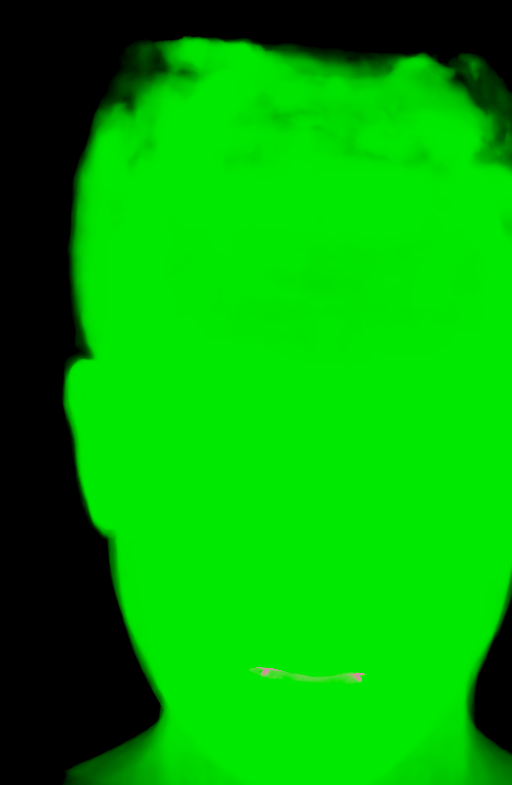
\includegraphics[height=\smallimageheight]{assets/\blendfieldsdirname/teaser2/colorsv2/0001.png}
        };
        \node[above right=\borderthickness and \borderthickness of training-2-3.south west, overlay]{
          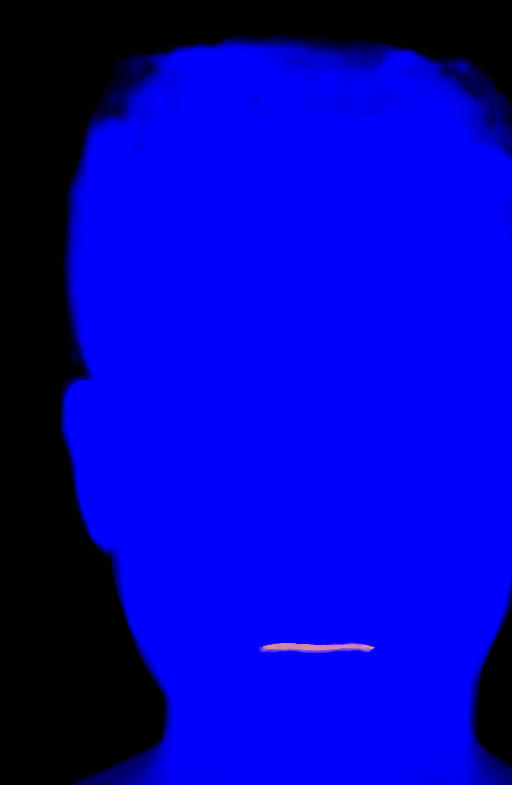
\includegraphics[height=\smallimageheight]{assets/\blendfieldsdirname/teaser2/colorsv2/0002.png}
        };
        \node[above right=\borderthickness and \borderthickness of training-2-4.south west, overlay]{
          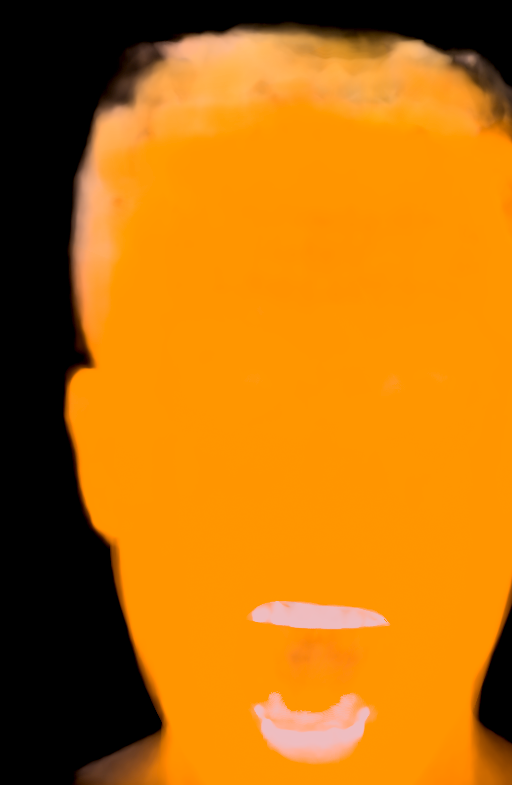
\includegraphics[height=\smallimageheight]{assets/\blendfieldsdirname/teaser2/colorsv2/0003.png}
        };
        \node[above right=\borderthickness and \borderthickness of training-2-5.south west, overlay]{
          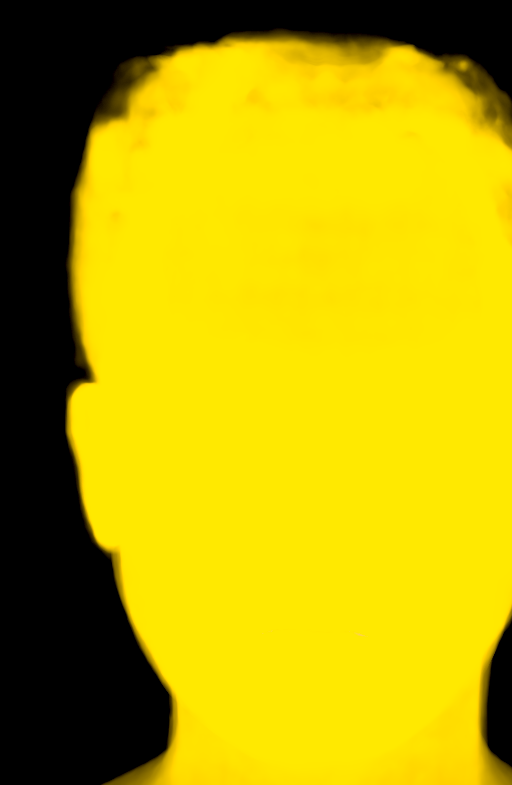
\includegraphics[height=\smallimageheight]{assets/\blendfieldsdirname/teaser2/colorsv2/0004.png}
        };

        \matrix[matrix of nodes, column sep=1pt, row sep=1pt, ampersand replacement=\&, right=1em of training, inner sep=0, outer sep=0] (final) {
          \includegraphics[height=\imageheight]{assets/\blendfieldsdirname/teaser2/voltemorph/final_markings.png} \\
          \includegraphics[height=\imageheight]{assets/\blendfieldsdirname/teaser2/ours/final_markings.png}       \\
        };
        \node[above right=\borderthickness and \borderthickness of final-2-1.south west, overlay]{
          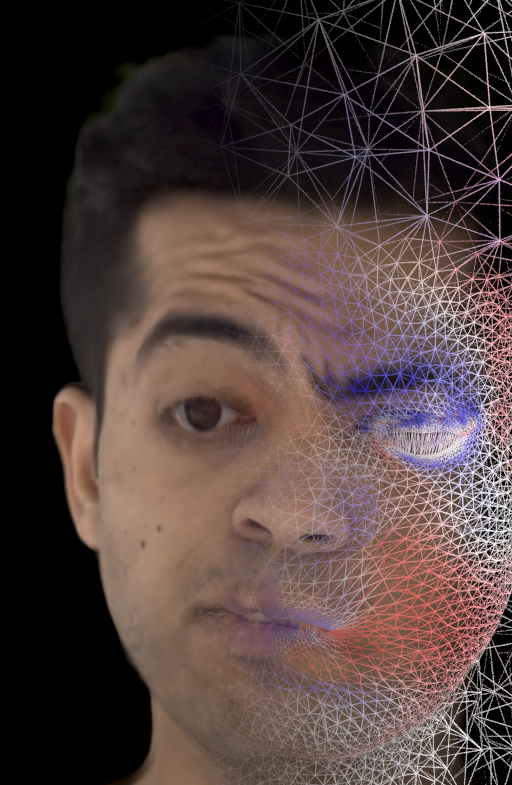
\includegraphics[height=\smallimageheight]{assets/\blendfieldsdirname/teaser2/colorsv2/final.png}
        };
        \node[above right=\borderthickness and \borderthickness of final-1-1.south west, overlay]{
          
\includegraphics[height=\smallimageheight]{assets/\blendfieldsdirname/teaser/colors/voltemorph.png}
        };

        % \node[below=0.25em of final-1-2] {\textbf{Ours}}; \node[below=0.25em
        % of final-1-1] {VolTeMorph \cite{garbin2022voltemorph}};
        % \node[left=0.75em of training-1-1.west, rotate=90, anchor=center]
        % {VolTeMorph \cite{garbin2022voltemorph}};
        \node[left=0.75em of training-1-1.west, rotate=90, anchor=center] {VolTeMorph};
        \node[left=0.75em of training-2-1.west, rotate=90, anchor=center] {\textbf{Ours}};
        % \draw[-] ($(training-1-1.south west)+(0.5em,-0.3em)$) -- node[below]
        % {Rendered training expressions} ($(training-1-5.south
        % east)+(-0.5em,-0.3em)$);
        \node[below=0.25em of training.south] {Rendered training expressions};
        \node[below left=0.25em and -2.5em of final-2-1.south] {Novel expression};

        \draw[densely dotted, line width=0.1em] ($(training-1-5.north east)+(0.5em,0.0em)$) -- ($(training-2-5.south east)+(0.5em,0.0em)$);

        % \matrix[matrix of nodes, inner sep=0, outer sep=0, column sep=0cm,
        % row sep=0cm, ampersand replacement=\&, right=1em of final]
        % (voltemorph) {

        % }; \draw[->,postaction={decorate,decoration={text along path,text
        % align=center,}}] (training-1-5.east) to [out=30,in=150]
        % (final-1-1.west);
      \end{tikzpicture}
    }
    % \includegraphics[width=\linewidth, height=8em]{example-image-a}
  \end{subfigure}
}

\newcommand{\blendfieldsteaserfigure}{
  \begin{figure}
    \centering
    \teasernobox
    \caption{
      \textbf{Teaser} --
      Given five multi-view frames of different expressions, our approach generates a model capable of capturing the fine-grained details of a novel expression beyond the resolution of the underlying face model~\cite{garbin2024voltemorph} (top right corner).
      This is achieved by \textit{blending} the radiance fields computed for
      individual expressions, where the blending coefficients are modulated
      accordingly to \textit{local} volumetric changes.
      These volumetric changes are measured as the difference in the
      tetrahedral volume of a mesh that deforms with the expression
      (\mycoloredbox{seismicred} increase, \mycoloredbox{seismicblue}
      decrease, and \mycoloredbox{seismicgray} no change in volume).
      Such an approach allows \textit{\blendfields} to render sharp,
      expression-dependent details of the face without increasing the
      resolution of the mesh (bottom right corner).
      \label{fig:blendfields-teaser}
    }
  \end{figure}

}
